grafik
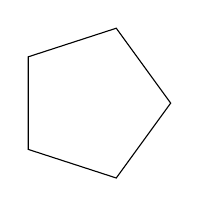
\begin{tikzpicture}
\draw (0:1cm) -- (72:1cm) -- (2*72:1cm) --
(3*72:1cm) -- (4*72:1cm) -- cycle;
\end{tikzpicture}

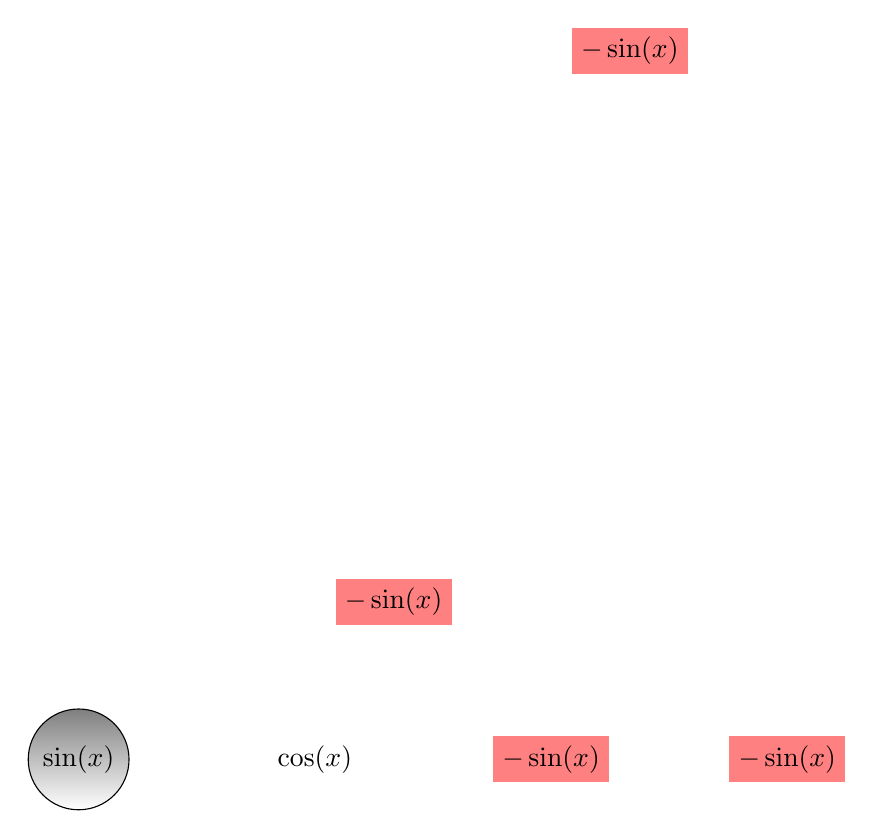
\begin{tikzpicture}
\node (A) at (0,0) [circle,shade,draw] {$\sin(x)$};
\node (B) at (3,0) {$\cos(x)$};
\node (C) at (6,0) [fill=red!50] {$-\sin(x)$};
\node (D) at (9,0) [fill=red!50] {$-\sin(x)$};
\node (E) at (4,2) [fill=red!50] {$-\sin(x)$};
\node (F) at (7,9) [fill=red!50] {$-\sin(x)$};
\end{tikzpicture}

\begin{tikzpicture}[
myrect/.style={
  rectangle,
  draw,
  inner sep=0pt,
  fit=#1}
]
\coordinate (A) at (2,3);
\coordinate (B) at (-3,4);
\coordinate (C) at (0,2);
\coordinate (D) at (-5,6);
\coordinate (E) at (5,-2);
\node[myrect={(A) (B)}] {}; 
\node[myrect={(C) (D)},draw=cyan,rounded corners] {}; 
\node[myrect={(A) (E)},draw=cyan,fill=orange,line width=2pt] {}; 
\foreach \Coord in {A,B,C,D,E}
  \node[circle,fill,inner sep=1.5pt,label=\Coord] at (\Coord) {};
\end{tikzpicture}